\chapter{Technical Foundation}\label{chap:technical-foundation}  % other option are Framework Design, Implementation Details

This chapter offers a comprehensive description of the context composition framework and the fine-tuning pipeline employed in the research presented in this thesis. Additionally, it includes a list of tools necessary for executing their implementations.

\section{Context Composition Framework}

This section begins with an explanation of the independent building blocks of the context composition framework and their integration to form a complete compositional strategy. It then enumerates all the composers utilized in the experimental section, accompanied by their descriptions. Finally, it offers an overview of the additional parameter applied to modify the retrieval order and includes a commentary that invites further exploratory investigation into the framework.

\subsection{Building Blocks}

As stated in \sectionref{sec:training-stages}, we define the context composer as a function that takes a repository snapshot and a completion file and returns a string that represents the project context. This function is decomposed into seven abstract blocks:

\begin{enumerate}
    \item \textbf{File Filtering} determines which files to include in the subsequent data processing pipeline. For instance, it can filter out files with empty content or files with certain extensions.
    \item \textbf{File Preprocessing} modifies the content of the files. For example, it can extract code from markdown files.
    \item \textbf{File Chunking} changes the granularity of the data from files to text chunks. The simplest form of chunking is identity, which maintains the file-grained structure.
    \item \textbf{Chunk Ranking} determines the relevance of the chunks for the completion file. It can take multiple forms, ranging from simple heuristics and sparse embedding comparisons to more sophisticated dense approaches.
    \item \textbf{Chunk Sorting} defines the rules for ordering the chunks based on their ranks. The most common scenario is to sort the chunks in ascending order of their ranks, placing the most relevant chunks at the end of the list.
    \item \textbf{Chunk Assembling} joins sorted chunks into a single string using a specific template. For example, the assembler can prepend a comment with path information of the chunk's source file and join them using a separator string.
    \item \textbf{Context Postprocessing} modifies the context as a unified string. For instance, line dropout can be applied by this block.
\end{enumerate}

Each of these blocks has its own abstract class and serves as a foundation for concrete implementations. This design allows for several different transformations associated with a single block type to be part of a single context composer, eliminates code duplication and allows for greater flexibility in composer creation. The directed graph presented in \figureref{fig:composer-blocks} visualizes the order in which these instances can be applied.

\begin{figure}[ht]
    \centering
    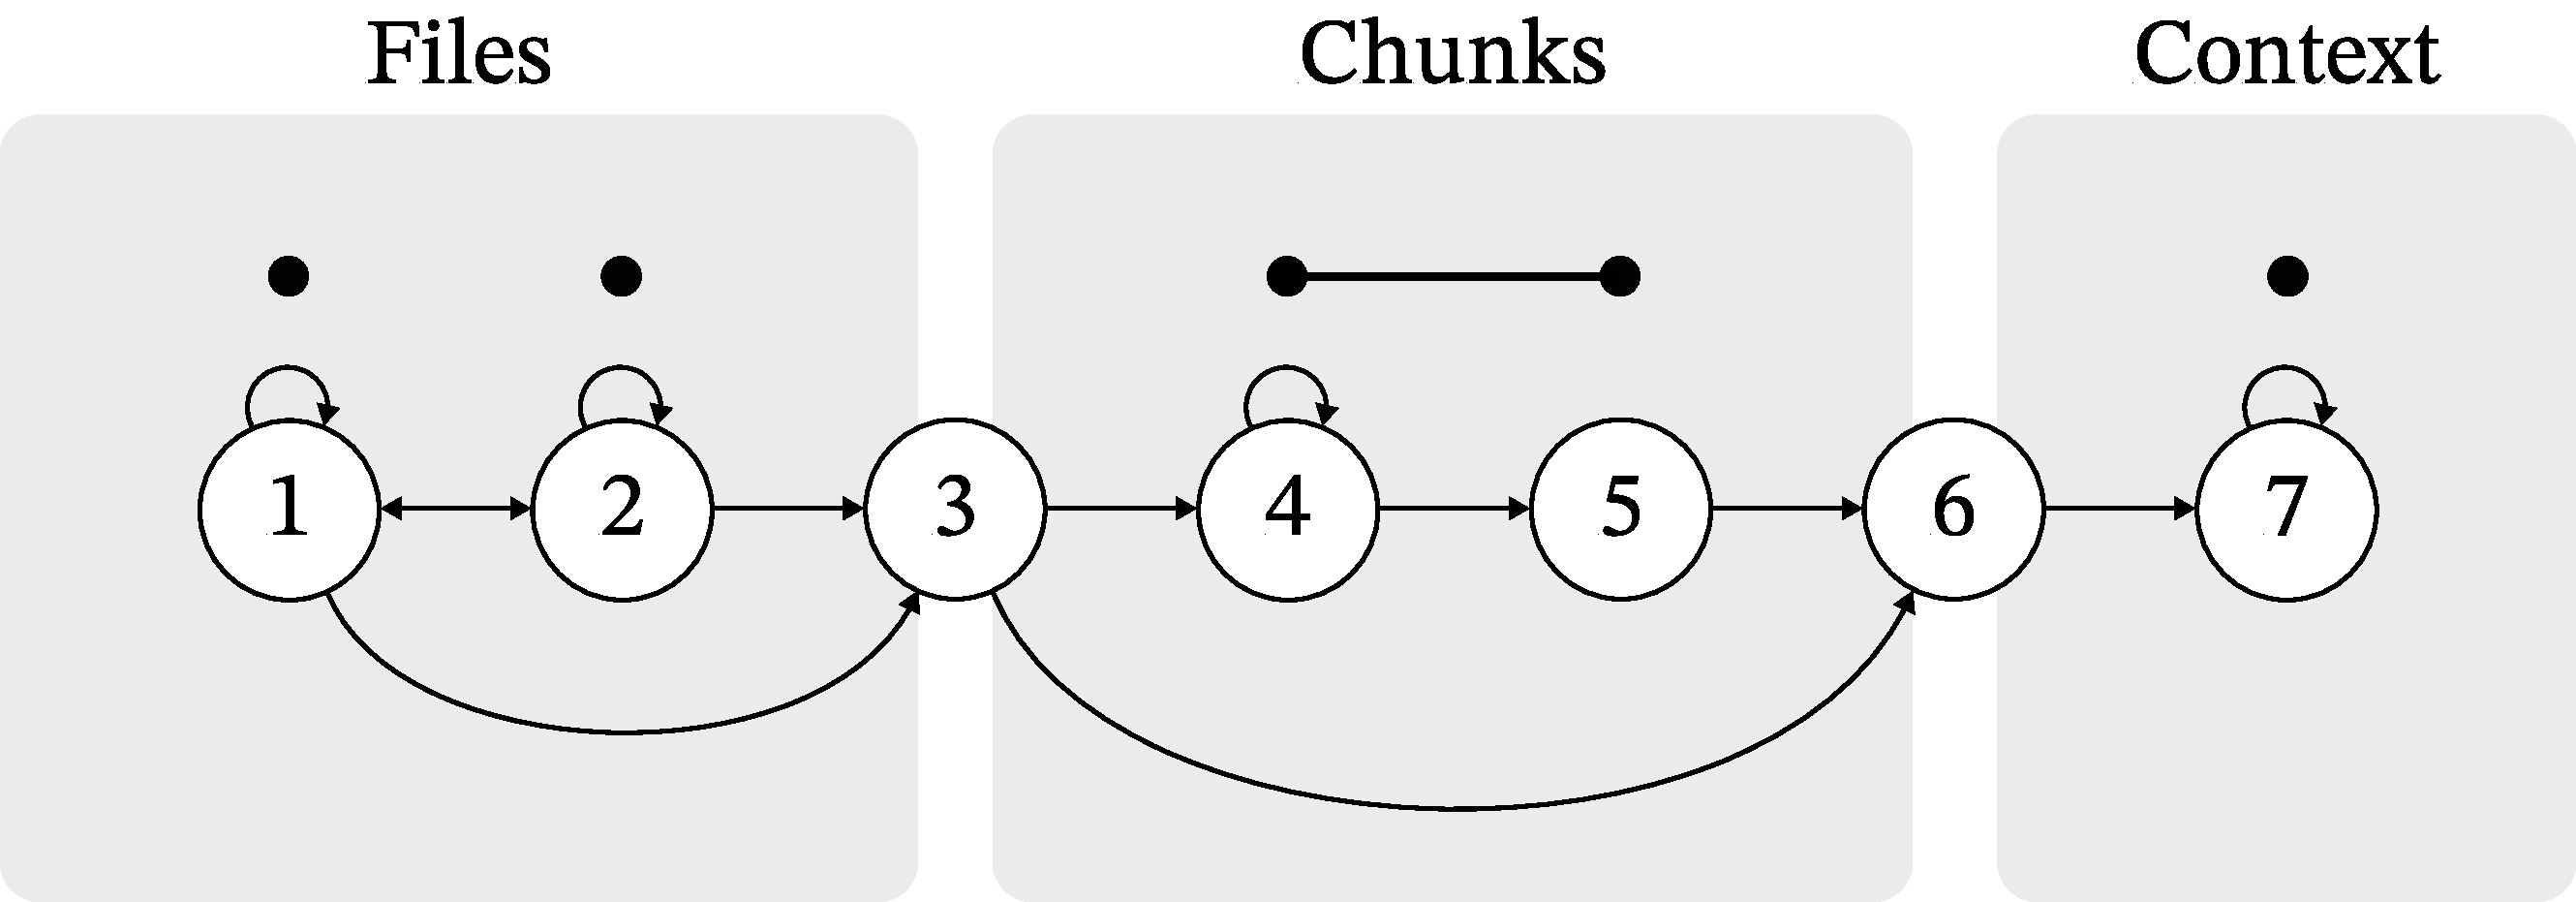
\includegraphics[width=\textwidth]{figures/composer-blocks.pdf}
    \caption{Order of composer blocks. Nodes represent block types: \textcircled{\raisebox{-0.9pt}{1}} File Filtering, \textcircled{\raisebox{-0.9pt}{2}} File Preprocessing, \textcircled{\raisebox{-0.9pt}{3}} File Chunking, \textcircled{\raisebox{-0.9pt}{4}} Chunk Ranking, \textcircled{\raisebox{-0.9pt}{5}} Chunk Sorting, \textcircled{\raisebox{-0.9pt}{6}} Chunk Assembling, and \textcircled{\raisebox{-0.9pt}{7}} Context Postprocessing. Edges indicate the permissible sequence of block application. The data format is denoted by three frames: Files, Chunks, and Context. The bold subgraph highlights blocks that may be omitted.}\label{fig:composer-blocks}
\end{figure}

\subsection{List of Context Composers}\label{sec:context-composers-list}

\begin{sloppypar}
All context composers utilized in the \nameref{chap:research-investigation} chapter adhere to two standard preprocessing steps: the removal of empty files and the normalization of all line endings to the Line Feed character. These shared preprocessing steps ensure consistency across all experiments. The following list provides a comprehensive overview of the context composers employed in this research.
\end{sloppypar}

\label{appendix:context-composers}
\begin{enumerate}
    \item \textbf{File-Level} produces an empty context.
    \item \textbf{Path Distance} constructs the context using only files with the \texttt{.py} extension. The selected files are sorted in descending order according to their path distance from the completion file. For files with identical path distances, a secondary sorting criterion is applied using the Intersection over Union (IoU) metric, which equals to the number of lines shared with the completion file divided by the total number of unique lines in both files. The IoU calculation considers lines with leading and trailing whitespace removed and includes only those lines that are at least five characters in length after whitespace removal.
    \item \textbf{Lines IoU} is similar to the Path Distance method, but omits the initial sorting by path distance. Instead, files are ranked directly using the IoU metric.
    \item \textbf{Code Chunks} removes all docstrings, comments, and import statements from the context produced by Path Distance.
    \item \textbf{Half-Memory} begins with the context generated by Path Distance. Each line is independently removed with a dropout probability of \(0.5\), maintaining the overall saturation of the context window.
    \item \textbf{Declarations} extends Path Distance by filtering out all non-declarative elements, retaining only function and class declarations.
    \item \textbf{Text Chunks} uses Path Distance as the base composer, but removes all code from the context, leaving only docstrings and comments.
    \item \textbf{Text Files} constructs the context using files with the extensions \texttt{.json}, \texttt{.yaml}, \texttt{.yml}, \texttt{.sh}, \texttt{.md}, \texttt{.txt}, and \texttt{.rst}. The selected files are grouped in ascending order of relevance: [\texttt{.json}], [\texttt{.yaml}, \texttt{.yml}], [\texttt{.sh}], [\texttt{.md}, \texttt{.txt}, \texttt{.rst}]. Within each group, files are further sorted in descending order according to their path distance from the completion file.
    \item \textbf{Random Files} constructs the context by randomly ordering all files from the repository snapshot.
    \item \textbf{Random \texttt{.py}} selects only files with the \texttt{.py} extension and arranges them in a random order.
    \item \textbf{Random Tokens} constructs the context by sampling a sequence of non-special tokens at random, with each token selected independently and with equal probability.
    \item \textbf{Duplication} constructs the context by repeatedly concatenating the content of the completion file until the maximum context window size is reached.
    \item \textbf{Leak} begins with the context produced by Path Distance. The completion file is randomly divided into five segments at newline characters, which then disjointedly replace context lines at random positions, approximately preserving the original token count.
\end{enumerate}\parencite{sapronov2025} % TODO: check the correctness of the citation
% TODO: motivate choices

\subsection{Order Modifications}

To increase the diversity of experiments conducted to address \hyperref[rq:rq-b1]{RQ.B1} and \hyperref[rq:rq-b2]{RQ.B2}, two additional file ordering modifications are considered alongside the \textit{original} mode, as illustrated in \figureref{fig:order-modes}:

\begin{itemize}
    \item \textit{reversed}: The retrieved files that fit within the model's context window are reordered in reverse. Consequently, the most relevant file appears at the beginning of the context window.
    \item \textit{irrelevant}: The order of retrieved files is reversed prior to the context length cut-off, resulting in a complete reversal of the context, with the most irrelevant files positioned at the end of the context string.
\end{itemize}

\begin{figure}[ht]
    \centering
    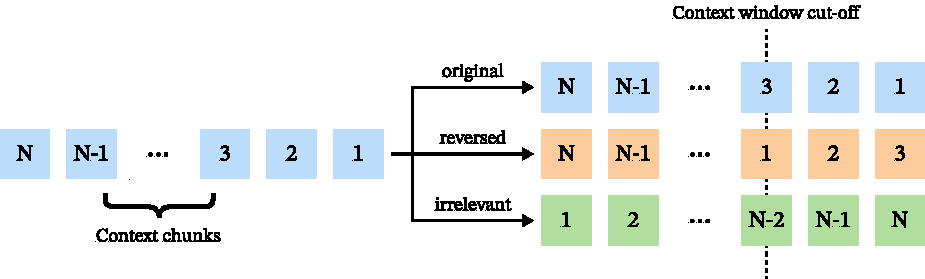
\includegraphics[width=\textwidth]{figures/order-modes.pdf}
    \caption{Three modes of context ordering. The numbers in boxes indicate the rank of the chunks, with smaller numbers denoting higher relevance.}\label{fig:order-modes}
\end{figure}

\subsection{Examples}

In addition to the blocks used to create composers employed in our experiments, we provide further exemplary implementations in the attached code, totaling 30 distinct blocks. The repository also includes a demonstrative Jupyter Notebook that describes these blocks and offers concrete usage examples of the package.

\section{Fine-Tuning Pipeline}

For the purposes of this research, we developed a fine-tuning pipeline aimed at adapting Code LLMs to the repository-level context.

From the data perspective, it supports the integration of pre-composed datasets obtained from the aforementioned context composition framework. The train-validation split is designed to eliminate data leakage from samples gathered from the same repositories. Configurable tokenization ensures context window saturation and facilitates the application of gradient masking.

The pipeline integrates models from the Hugging Face Hub\footnote{\url{https://huggingface.co/}}. It supports adapters that can augment the model architecture, freeze a subset of parameters, or modify the optimizer initialization. Models are dynamically loaded onto a single device based on hardware availability. Efficient attention implementation and parameter data types are selected using the same principle.

The training loop is implemented in pure PyTorch\footnote{\url{https://pytorch.org/}}. It supports cosine learning rate scheduling with linear warmup, gradient scaling, clipping, and accumulation. The pipeline can periodically invoke two validation loops: one on the original dataset split and another on an additional provided dataset. The latter allows metrics to be grounded on baseline composition strategy instead of solely monitoring the in-distribution capabilities of the model.

During the training process, the pipeline produces a set of configurable metrics and statistics for both the training and validation data. These include cross-entropy, Exact Match, Top-\(k\) Accuracy, learning rate tracking, epoch and token number counting. Their values are decomposed based on the types of tokens they are applied to. We denote five such types:
\begin{itemize}
    \item \textbf{Attached:} Tokens whose losses participate as leaf nodes in automatic differentiation for gradient computation.
    \item \textbf{Detached:} Tokens whose losses are zeroed out during gradient masking and serve as a complement to the attached tokens.
    \item \textbf{Completion:} Tokens of the completion file.
    \item \textbf{Context:} Tokens of the repository context.
    \item \textbf{Full:} All tokens.
\end{itemize}

In addition to statistics and metrics, the pipeline provides logging of the standard output and error streams. Checkpointing of the model and optimizer states is also supported.

The entire pipeline utilizes a modular structure, which enhances code maintainability and extendability. It is designed in an end-to-end manner, requiring only a pre-composed dataset, a set of YAML configuration files, and a single command line from the user. All components that employ stochastic behavior are accompanied by a seed parameter, ensuring that all experiments are reproducible.

\section{Tools}

In the context composition framework, we integrate Hugging Face tokenizers from the Transformers\footnote{\url{https://github.com/huggingface/transformers}} library to compute token-related statistics, and Tree-sitter\footnote{\url{https://tree-sitter.github.io/tree-sitter/}} to decompose Python code into its parts. Both libraries are employed in the concrete implementations of the blocks, although their usage can be omitted without disrupting the main abstract framework. The OmegaConf\footnote{\url{https://github.com/omry/omegaconf}} configuration system is utilized to manage the initialization of the composers from YAML configuration files.

The pipeline inherits requirements from the context composition framework as it utilizes its functions. Additionally, it employs Datasets\footnote{\url{https://github.com/huggingface/datasets}} and Accelerate\footnote{\url{https://github.com/huggingface/accelerate}} from the Hugging Face ecosystem to provide peripheral support to the Transformers library. The Hydra\footnote{\url{https://github.com/facebookresearch/hydra}} package extends the configurative capabilities of OmegaConf and enhances the pipeline's usability. PyTorch, as mentioned in the previous section, is used to implement the training loop. The tqdm\footnote{\url{https://github.com/tqdm/tqdm}} library is employed to display progress bars for all prolonged processes. Weights~\&~Biases\footnote{\url{https://github.com/wandb/wandb}} is used to track metrics and statistics in real-time.

% TODO: add Pandas

To conduct all experiments and run evaluation scripts, a single 8\(\times\)H200 node was used, with each GPU having 141 GB of VRAM.
